% res_numerics.tex  -- written by Harshvardhan
\subsection{Numerical Accuracy}
Table~\ref{tab:num} compares the fixed-point datapath with float64 over
5000 random products per input distribution. The accumulator itself adds
no error: all error comes from quantising the inputs to Q4.4 (RMSE
0.030 for uniform$[-1,1)$). Requantising to Q4.4 adds only rounding error,
about $0.0625/\sqrt{12}$ per element, giving an RMSE of 0.035
(Fig.~\ref{fig:num}). For larger inputs (uniform$[-2,2)$), 0.3\,\% of the
outputs exceed $\pm8$ and saturate; the \texttt{sat} flags report this to
the host. A Q8.8 output never saturated in these tests.

\begin{table}[t]
\centering
\caption{Accuracy vs.\ float64 (5000 products per distribution)}
\label{tab:num}
\setlength{\tabcolsep}{3pt}
\begin{tabular}{@{}lrrrr@{}}
\toprule
\textbf{Inputs} & \textbf{RMSE Q24.8} & \textbf{RMSE Q4.4} & \textbf{max err Q4.4} & \textbf{sat.\ Q4.4}\\
\midrule
uniform$[-1,1)$ & 0.0295 & 0.0346 & 0.159 & 0.00\,\% \\
uniform$[-2,2)$ & 0.0591 & 0.0617 & 0.255 & 0.30\,\% \\
normal$(0,0.5)$ & 0.0255 & 0.0312 & 0.145 & 0.00\,\% \\
\bottomrule
\end{tabular}
\end{table}

\begin{figure}[t]
\centering
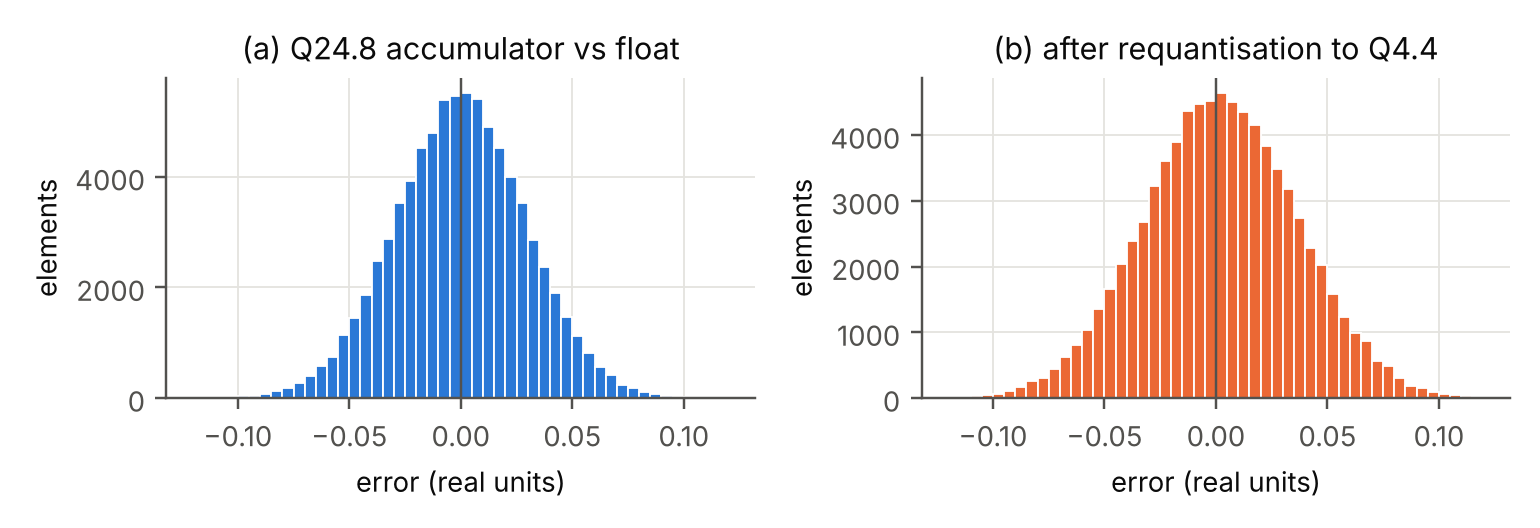
\includegraphics[width=\columnwidth]{fig_numerics.png}
\caption{Error distribution vs.\ float64, uniform$[-1,1)$ inputs.}
\label{fig:num}
\end{figure}
